\documentclass[12pt,a4paper]{report} 
\usepackage[utf8]{inputenc}
\usepackage{amsmath}
\usepackage{graphicx}
\usepackage{wrapfig}
\usepackage{listings}
\usepackage{minted} 
\usepackage{mathtools}
\usepackage{fancyvrb, listings, color}

\DeclarePairedDelimiter\ceil{\lceil}{\rceil}
\DeclarePairedDelimiter\floor{\lfloor}{\rfloor}

\usepackage{tikz,fouriernc}
\usetikzlibrary{calc}
\definecolor{lime}{RGB}{0,0,20}

\date{}

\begin{document}
    \begin{titlepage}
        \begin{tikzpicture}[overlay,remember picture]
            \fill[lime!10] (current page.south east) rectangle (current page.north west);
            \fill[lime,even odd rule] (current page.south west) rectangle ([xshift=1.5cm]current page.north west) ($(current page.north west)!.5!(current page.south west)$) arc(180:270:3) ($(current page.north west)!.5!(current page.south west)$) arc(270:450:3.5) ([yshift=7cm]$(current page.north west)!.5!(current page.south west)$)  arc(180:90:3);
%           \draw[lime!10,double=lime!10,double distance=2mm] (current page.south west) --+ (2,2) --+ (-2,6) --+ (2,8) --+ (-2,9) --+ (2,13) --+ (-2,18) --+ (2,30);
            \node[yshift=-5cm,lime] at (8,-7) {\scalebox{4}{Graphs and}};
            \node[yshift=-7cm,lime] at (8,-7) {\scalebox{4}{Number Theory}};
                \draw[lime,fill=lime!20] ([xshift=-1cm]current page.north east) -- ([yshift=-1cm]current page.north east) -- ([yshift=-2cm]current page.north east) -- ([xshift=-2cm]current page.north east);
            \path ([xshift=-1cm]current page.north east) -- ([yshift=-1cm]current page.north east) node[midway,sloped,below=.2cm,lime] {Yash Bhatia};
        \end{tikzpicture}
    \end{titlepage}
\tableofcontents
\chapter{Graph Basics}

\section{Introduction}
A graph is a data structure made up of nodes and edges that is non-linear. The edges are lines or arcs that link any two nodes in the graph, and the nodes are also known as vertices. A graph can be described more formally as: A Graph consists of a finite set of vertices(or nodes) and set of Edges which connect a pair of nodes.In this chapter, we will look at the most basics techniques that are employed in most graph algorithms.

\section{Depth First Search}
The depth-first search technique is used to traverse or explore data structures such as trees and graphs. The algorithm starts from the root node (in the case of a graph, any random node can be used as the root node) and examines each branch as far as feasible before retracing. So the fundamental concept is to start at the root node and mark it visited. Then, we do a recursive traversal over the children until all the vertices are visited.\\
We maintain a boolean array to keep a track of the already visited noes. Then we check the adjacency list of that node. If we find that any node is unvisited, we start dfs from that node, and the above described process repeats.\clearpage
\begin{minted}
[
frame=lines,
framesep=2mm,
baselinestretch=1.2,
fontsize=\footnotesize,
linenos
]
{cpp}

void dfs(int ver, bool vis[])
{   
    vis[ver] = true;
    for(auto &i : ver)
    {
        if(!vis[i])
        {
            dfs(i,vis);
        }
    }
}
\end{minted}


\section{Breadth First Search}
One of the most basic and important graph searching methods is breadth first search.The path found by breadth first search to any node is the shortest path to that node, i.e. the path with the lowest number of edges in unweighted networks, as a result of how the process works.The algorithm starts with some start vertex $s$ which is pushed into a queue. What we want to do is : Discover all the nodes at a particular depth first before moving to the next level. 
\begin{minted}
[
frame=lines,
framesep=2mm,
baselinestretch=1.2,
fontsize=\footnotesize,
linenos
]
{cpp}
queue<int> q;
bool used[n];   // Visited array
vector<int> d(n);
q.push(s);
used[s] = true;
while (!q.empty()){
    int v = q.front();
    q.pop();
    for (int u : adj[v]) {
        if (used[u] == false) {
            used[u] = true;
            q.push(u);
            d[u] = d[v] + 1;
        }
    }
}
\end{minted}


So what we do is, we start from this source vertex, and push all its children into the queue. We then pop off this node. Then we push all the children of the top of stack into the queue and then pop off this node. We keep repeating this process until the queue isn't empty. We also ensure that no node is visited twice.\\
To ensure that no node is visited twice, we maintain a boolean array. Every time we push a node into the queue, we set the visited value of that node to true. If the child in a particular iteration is already visited, we do nothing. \\
BFS can be very useful in finding the depth of a particular node. The above program is a good description of that. (Depth might not make a lot of sense in general graphs, so assume its a tree). Whenever we push a child onto the queue, we set its depth equal to its parent's depth + 1
\chapter{Shortest Path Algorithms}

\section{Introduction}
This is a very basic, yet important topic of graph theory. This has many real life applications such as: finding the shortest route between two cities, minimum cost of wiring, etc. Digital mapping services in Gmaps, telephone networks, IP routing are some places where we use shortest path algorithms. Shortest path algorithms are mainly classified into two: Single source shortest path and Multiple source shortest path.

\section{Single Source Shortest Path}
As the name suggests, we have once source node $S$ , and we find the minimum distance from this node to any other node in the graph.

\subsection{Dijkstra }
Let's make an array $d[|V|+1]$ in which we record the current length of the shortest path from s to $v$ in $d[|V|+1]$ for each vertex v. Initially, $d[S]=0$, and this length equals infinity for all other vertices. In the implementation a sufficiently large number (which is guaranteed to be greater than any possible path length) is chosen as $\infty$.\\
In addition, we maintain a Boolean array $u[|V|+1]$ which stores for each vertex $v$ whether it's marked. Initially all vertices are unmarked. \\
The Dijkstra algorithm iterates for n times. Each iteration, an unmarked vertex v with the lowest value d[v] is chosen as the unmarked vertex.
\begin{minted}
[
frame=lines,
framesep=2mm,
baselinestretch=1.2,
fontsize=\footnotesize,
linenos
]
{cpp}
vector<int> d (num_vertices+1, INF);
void dijkstra()
{
    priority_queue <pii, vector<pii>, greater<pii> > pq;
    pq.push({0,S});
    d[S] = 0;
    while(!pq.empty())
    {
        int x = pq.top().second;
        pq.pop();
        if(vis[x] == true)
            continue;
        vis[x] = true;
        for(auto i:v[x])
        {
            int ver = i.first;
            ll len = i.second;
            if(d[ver] == d[x] + len)
            {
                num[ver]++;
            }
            else if(d[ver] > d[x] + len)
            {
                num[ver] = 1;
                d[ver] = d[x] + len;
                pq.push({d[ver],ver});
            }
        }
    }
}
\end{minted}

Obviously, the start vertex $S$ will be chosen in the first iteration.Following that, relaxations from vertex v are performed: all edges of the type $(v,\text{to})$ are evaluated, and the method tries to improve the value $d[{to}]$ for each vertex. If the current edge's length equals $\text{len}$, the relaxation code is:
$$
    d[\text{to}]=\text{min}(d[\text{to}],d[v]+\text{len})
$$
The current iteration finishes after all such edges have been examined. After $n$ iterations, all of the vertices will be relaxed.

\subsection{Bellman Ford}
Unlike the Dijkstra algorithm, this algorithm can also be applied to graphs containing negative weight edges . However, if the graph contains a negative cycle, then, clearly, the shortest path to some vertices may not exist (due to the fact that the weight of the shortest path must be equal to minus infinity); however, this algorithm can be modified to signal the presence of a cycle of negative weight, or even deduce this cycle.\\
For now, let's assume that the graph doesn't have negative cycles. We will create an array of distances $d[1 \cdots n]$, which after execution of the algorithm will contain the answer to the problem. In the beginning we fill it as follows: $d[S]=0$, where $S$ is the source vertex and all other elements equal to $\infty$.\\
We perform the following procedure $n-1$ times : traverse through all the edges of the graph and relax the destination node. In other words $d(v) = \text{min}(dist[u] + l(u,v))$. We claim that the final distance array is the solution to the single source shortest path problem. But why do we run this $n-1$ times? It's simple - Realize that the shortest path between any two nodes takes atmost $n-1$ edges. So relaxing each edge $n-1$ times is enough. Here's a pseudocode:
\begin{minted}
[
frame=lines,
framesep=2mm,
baselinestretch=1.2,
fontsize=\footnotesize,
linenos
]
{cpp}
vector<int> d (num_vertices+1, INF);
void BellmanFord()
{
    d[v] = 0;
    for (int i=0; i<n-1; ++i)
        for (int j=0; j<num_edges+1; ++j)
            if (d[e[j].a] < INF)
                d[e[j].b] = min (d[e[j].b], d[e[j].a] + edg[j].cost);
}
\end{minted}

To detect negative cycles, simply run this algorithm for $n-1$ more times, and check whether any value in $d$ array changes. If it does, then there does exist a negative cycle.

\section{Multiple Source Shortest Path}
Now, we need to find the minimum distance between any pair of vertices. For this, we use the famous Floyd Warshall algorithm. This algorithm uses dynamic programming, and is surprisingly much easier than the ones we learnt.

\subsection{Floyd Warshall}
The Floyd Warshall Algorithm is used to solve the issue of finding the shortest path between two pairs of verticees. The goal is to discover the shortest distance between each pair of vertices in an edge-weighted directed Graph.\\
Dijkstra isn't relevant because we're taking into account even the negative edges. Bellman-Ford, on the other hand, would result in a $O(V^4)$ complexity that is exceedingly low. The complexity of this approach is reduced to $O(V^3)$ using Dynamic Programming.\\
We define the following DP state: Let $f(i,j,k)$ be the shortest path from node $i$ to node $j$ that uses only the vertices $1,2,3,\cdots,k$ as intermediates. 

We define the transition state as follows :
$$
f(i,j,k) = \text{min}(f(i,j,k-1) , f(i,k,k-1)+f(k,j,k-1))
$$
This is because, we can either include or exclude the $k^{th}$ vertex as an intermediate. We calculate the answer in both cases, and return the minimum.

We can see that this would require both :

$\text{Time Complexity = } O(V^3)$

$\text{Space Complexity = }O(V^3)$\\
However, we can improve the space complexity here. Rather than creating a $3D$ array, for storing each of the $2D$ arrays of a given dimension, we can keep updating the $2D$ array itself, as we backtrack by just one step. This reduces $\text {Space Complexity to }O(V^2)$. Have a look at the pseudocodde:
\begin{minted}
[
frame=lines,
framesep=2mm,
baselinestretch=1.2,
fontsize=\footnotesize,
linenos
]
{python}
for i in range(1,n+1):
    for j in range(1,n+1):
        dp[i][j] = INFINITY
for all (i,j) in E:
    dp[i][j] = length(i,j)
for k in range(1,n+1):
    for i in range(1,n+1):
        for j in range(1,n+1):
            dp[i][j] = min(dp[i][k] + dp[k][j] , dp[i][j])
\end{minted}
\chapter{Lowest Common Ancestor}
\section{Introduction}
The Lowest Common Ancestor (LCA) of two nodes $v$ and $w$ in a tree or directed acyclic graph (DAG) $T$ is the lowest (i.e. deepest) node that includes both v and w as descendants, where each node is defined as a descendent of itself in graph theory and computer science (so if $v$ has a direct connection from $w$, $w$ is the lowest common ancestor).In the development of object-oriented programming systems, the challenge of determining lowest common ancestors of classes in an inheritance hierarchy arises.The LCA problem also has applications in distributed computing models of complex systems.

\section{$k^{th}$ ancestor}
We need to solve the following problem: Given a tree with $N$ nodes, answer $Q$ queries. The $i^{th}$ query will contain two integers $a_i,b_i$ where $a_i$ is a node of the tree. The answer to the $i^{th}$ query is a node $p$ , such that $p$ is the $b_i^{th}$ ancestor of node $a_i$.\\
The naive approach to solve this problem would be to store the parent of each node in an array, and to run a simple for loop to find the $k^{th}$ ancestor. The worst case time complexity of this approach would be $O(N)$ for each query, and hence the overall complexity will be $O(NQ)$. Now, ofcourse it's time to ask the most clichéd question - Can we do better?\\
Let's try to come up with some possible approach to solve this.\\
\clearpage
\subsection{Idea for Binary Lifting}
Let's assume that for every node $x$, we know all the ancestors of $x$ that are perfect powers of two. That means, we know the $1^{st} , 2^{nd}, 4^{th} , 8^{th} \cdots$ ancestors of node $x$.Can we somehow use this data to find any ancestor of node $x$? Well, let's see: \\
Let's say we want to find the $6^{th}$ ancestor of node $x$. Let's say, $y$ is the $4^{th}$ ancestor of node $x$. Realize that,\\
\begin{figure}[h]
    \centering
    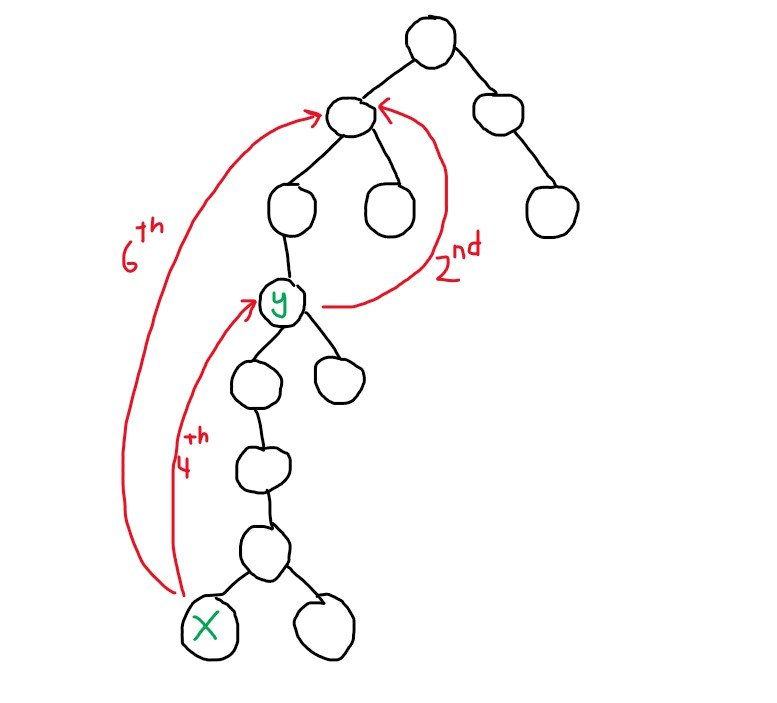
\includegraphics[scale=0.5]{images/lifting.jpg}
    \caption{Binary Lifting}
    \label{fig:my_label}
    
\end{figure}
\\ $$6^{th} \text{ancestor of node x} = 2^{nd} \text{ancestor of node y}$$

You might have already realized what to do by now. Let $b[i]$ represent the $i^{th}$ bit of number x. If the $i^{th}$ bit is set, i.e. $b[i] = 1$, then find the $2^{i}$th ancestor of node $x$, and reset the value of $x$ such that $x = 2^{i}\text{th ancestor of x}$. \\
For example, the bitwise representation of $14$ is $1110$. So, find the $8^{th}$ ancestor of $4^{th}$ ancestor of $2^{nd}$ ancestor of node $x$, and that shall be our final answer.\\
For some reason, I always refer to this method as "Anti Divide and Conquer" (unofficial). This is because - unlike divide and conquer, where we divide the problem into powers of two - we build up the powers of two solve this problem. Anyways, we considered the powers of two ancestors as black box. Now, we shall look at how to build these powers of two.

\subsection{Algorithm for Binary Lifting}
Let's see how to find the powers of two ancestors first:\\

\begin{minted}
[
frame=lines,
framesep=2mm,
baselinestretch=1.2,
fontsize=\footnotesize,
linenos
]
{cpp}
void dfs(int ver)
{
    vis[ver] = true;
    for(int i=1; i<30; i++)
    {
        if(ancestor[ver][i-1] != -1)
            ancestor[ver][i] = ancestor[ancestor[ver][i-1]][i-1];
        else
            ancestor[ver][i] = -1;
    }
    for(auto &i : v[ver])
    {
        if(vis[i] == false)
        {
            ancestor[i][0] = ver;
            depth[i] = depth[ver] + 1;
            dfs(i);
        }
    }
}
\end{minted}
This is an application of dynamic programming which works as follows: $\text{ancestor}[i][j]$ is the $2^j{th}$ ancestor of node $i$.We set $\text{ancestor}[\text{root}][0] = -1$. When we iterate through the children of node $i$, we set $\text{ancestor}[\text{child of } i][0] = i$. \\
Then we use the following rule to find the $2^{j}$th ancestor:\\
\begin{equation*}
    \text{ancestor}[i][j]=
    \begin{cases}
      \text{ancestor}[\text{ancestor}[i][j-1]][j-1], & \text{if}\ \text{ancestor}[i][j-1] != -1 \\
      -1, & ,\text{otherwise}
    \end{cases}
\end{equation*}
While doing so, also compute the depth of each node. The reason shall be explained later. \clearpage

Now we see how to compute the $k^{th}$ ancestor.\\
\begin{minted}
[
frame=lines,
framesep=2mm,
baselinestretch=1.2,
fontsize=\footnotesize,
linenos
]
{cpp}
int kthancestor(int v, int k)
{
    int node = v;
    for(int i=0; i<30; i++)
    {
        if(k & (1 << i))
            node = ancestor[node][i];
    }
    return node;
}
\end{minted}

As discussed earlier, we find the bitwise representation of $k$.  Let $b[i]$ represent the $i^{th}$ bit of number $k$. If the $i^{th}$ bit is set, i.e. $b[i] = 1$, then find the $2^{i}$th ancestor of node $x$, and reset the value of $k$ such that $k = 2^{i}\text{th ancestor of x}$.

\subsection{Complexity Analysis}
Excluding precomputation time for powers of two (which takes $O(N \logN)$), each query takes $O(\log N)$ time. So, the overall time complexity is $O(Q \log N)$. Space complexity would be $O(N \log N)$ for the ancestor array.
\clearpage
\section{Lowest Common Ancestor(LCA)}
Problem Statement: Given two nodes $u$ and $v$ of a tree, find a node $w$, such that $w$ is the node with highest depth, having both $u$ and $v$ as it's descendants.\\
Now that we know how to find the $k^{th}$ ancestor of a node, this is rather simple.Remember, we included a depth[ ] array earlier in the dfs() code? This is where we will use it. The first obvious step would be to bring $u$ and $v$ to the same level. Without any loss of generality, $\text{depth}[u] \ge \text{depth}[v]$.\\
So, the difference in their levels would be $x = \text{depth}[u] - \text{depth}[v]$. 
\begin{figure}[h]
    \centering
    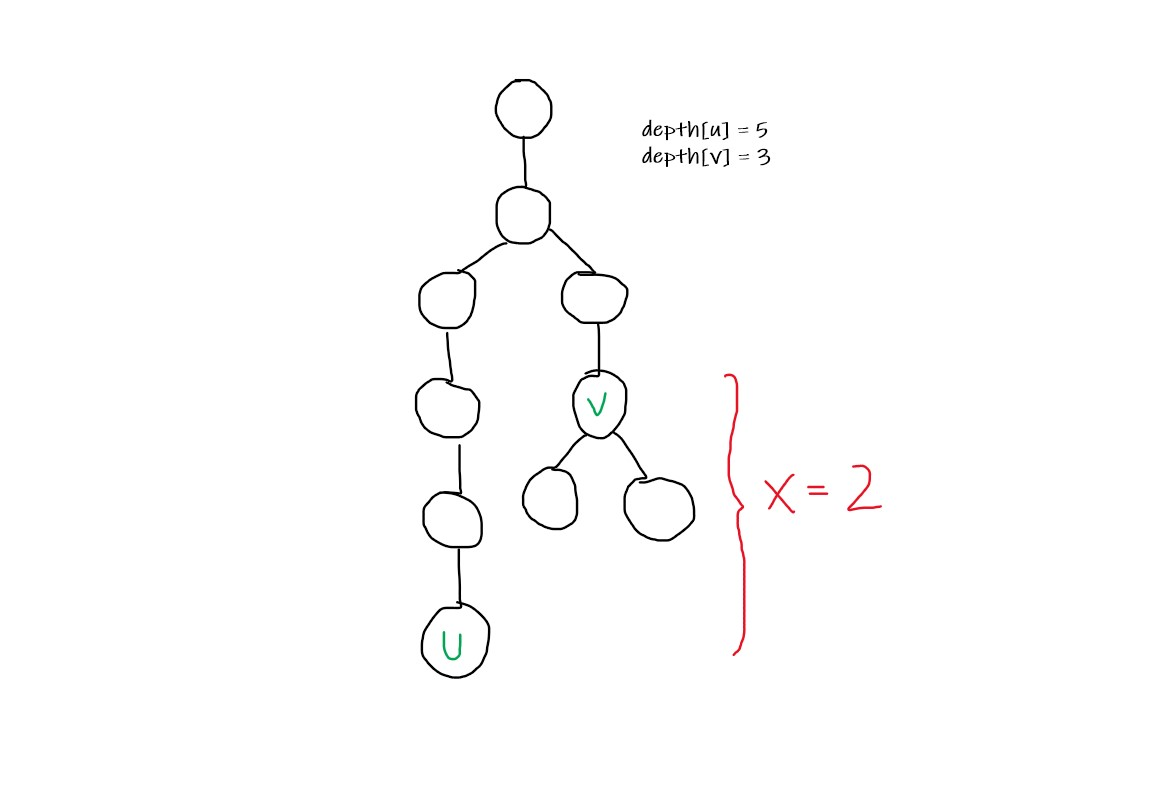
\includegraphics[scale=0.6]{images/lca.jpg}
    \caption{LCA}
    \label{fig:my_label}
\end{figure}
Now that $u$ and $v$ are at the same level, let's say $k^{th}$ ancestor of $u$ (and $v$) is the LCA. Then, $\forall p \in [k,\infty)$ , the $p^{th}$ node is also a common ancestor. So, starting from the MSB, we find the highest bit such that the ancestors of $u$ and $v$ are not common, and move it upto that level accordingly. 
The code would look as follows:
\begin{minted}
[
frame=lines,
framesep=2mm,
baselinestretch=1.2,
fontsize=\footnotesize,
linenos
]
{cpp}
int LCA(int a, int b)
{
    if(depth[a] < depth[b])
        swap(a,b);
    a = kthancestor(a , depth[a] - depth[b]);
    if(a == b)
        return a;
    for(int i=30; i>=0; i--)
    {
        if(ancestor[a][i] != ancestor[b][i])
        {
            a = ancestor[a][i];
            b = ancestor[b][i];
        }
    }
    return ancestor[a][0];    
}
\end{minted}
\subsection{Complexity Analysis}
The time and space complexity would be the same as binary lifting, i.e. $O(N \log N$) each.

\chapter{Convex Hull}
\section{Introduction}
Given a set of points in the plane. the convex hull of the set is the smallest convex polygon that contains all the points of it. There are many different algorithms to find the convex hull. We will mainly focus on the two most famous ones : Jarvis March and Graham's scan.  

\section{Right Hand Thumb Rule}
\begin{wrapfigure}{R}{0.3\textwidth}
\centering
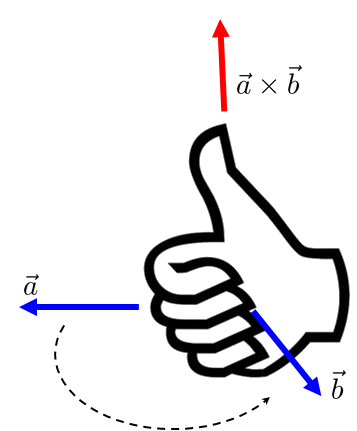
\includegraphics[width=0.25\textwidth]{images/rhtr.png}
\caption{\label{fig:frog1}Right hand thumb rule}
\end{wrapfigure}

The conventional criterion for right-handedness of screws is to curl your right hand's fingers around it while running your thumb along it. It's right-handed if it screws in (in the direction of your thumb) when twisted in the direction your fingers point.

The right hand rule for rotation vectors works on the same principle: curl your right hand's fingers in the rotation's direction. If it isn't possible, rotate your wrist until it is. The rotation vector is then determined by the direction of your thumb.

Anyways, why do we need this? We will very soon realize that we need some tool to get a sense of clockwise and anticlockwise directions to find the convex hull. We say that the angle is clockwise if cross product is positive, while anticlockwise if its negative. In other words, if we want to go from $\vec{a}$ to $\vec{b}$ and $\vec{a} \times \vec{b}$ is positive, then we have to go clockwise, else anticlockwise. \clearpage
\section{Template}
We will use the below template for convex hull, and any other geometry problem later.
\begin{minted}
[
frame=lines,
framesep=2mm,
baselinestretch=1.2,
fontsize=\footnotesize,
linenos
]
{cpp}
template <class T> int sgn(T x) { return (x > 0) - (x < 0); }
template<class T>
struct Point {
	typedef Point P;
	T x, y;
	explicit Point(T x=0, T y=0) : x(x), y(y) {}
	bool operator<(P p) const { return tie(x,y) < tie(p.x,p.y); }
	bool operator==(P p) const { return tie(x,y)==tie(p.x,p.y); }
	P operator+(P p) const { return P(x+p.x, y+p.y); }
	P operator-(P p) const { return P(x-p.x, y-p.y); }
	P operator*(T d) const { return P(x*d, y*d); }
	P operator/(T d) const { return P(x/d, y/d); }
	T dot(P p) const { return x*p.x + y*p.y; }
	T cross(P p) const { return x*p.y - y*p.x; }
	T cross(P a, P b) const { return (a-*this).cross(b-*this); }
	T dist2() const { return x*x + y*y; }
	double dist() const { return sqrt((double)dist2()); }
	double angle() const { return atan2(y, x); }
	bool null() const { return (x == 0 && y == 0); }
	P unit() const { return *this/dist(); } // makes dist()=1
	P perp() const { return P(-y, x); } // rotates +90 degrees
	P normal() const { return perp().unit(); }
	P rotate(double a) const {
		return P(x*cos(a)-y*sin(a),x*sin(a)+y*cos(a)); }
	friend ostream& operator<<(ostream& os, P p) {
		return os << "(" << p.x << "," << p.y << ")"; }
};
\end{minted}
\section{Jarvis March}
This is probably the most obvious non-brute algorithm that most people would come up with.
\begin{figure}[h]
    \centering
    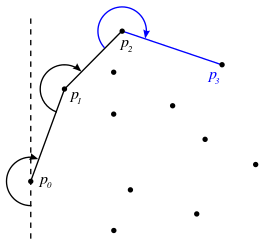
\includegraphics[scale=0.4]{images/jarvis.png}
    \caption{Jarvis Hull}
    \label{fig:my_label}
    
\end{figure}
We start by selecting one point that will definitely be a part of the convex hull. This can be one of the $X$ or $Y$ extremes. Let's say we select the leftmost point. Let's say we want move in a clockwise fashion. So, for any given point, we check for a point which is the leftmost. In other words, if we join the initial and final points, then the cross product of this vector with any other vector (with the same initial point) is non-positive.
The code for this would look as follows:
\begin{minted}
[
frame=lines,
framesep=2mm,
baselinestretch=1.2,
fontsize=\footnotesize,
linenos
]
{cpp}
using P = Point<int>;
vector<P> jarvisMarch(vector<P> pts) {
	int l = 0;
    vector<P>convex_hull;
    for(int i=0; i<pts.size(); i++)
        if(pts[i].y < pts[l].y)
            l = i;
    int pt = l;
    int ch;
    do{
        convex_hull.push_back(pts[pt]);
        ch = (pt+1)%(pts.size());
        for(int i=0; i<pts.size(); i++)
        {
            if((pts[i] - pts[pt]).null())continue;
            if((pts[ch] - pts[pt]).cross(pts[i] - pts[pt]) < 0)
                ch = i;
            else if((pts[ch] - pts[pt]).cross(pts[i] - pts[pt]) == 0)
                if((pts[ch] - pts[pt]).dist() < (pts[i] - pts[pt]).dist())
                    ch = i;
        }
        pt = ch;
    } while (pt != l);
    return convex_hull;
}
\end{minted}
\subsection{Complexity Analysis}
Let's say the convex hull has $m$ edges. Then the worst case time complexity is $O(nm)$. So, if we somehow know that the hull would have less number of edges, then this is a good method. The average time complexity is around $O(n \log n)$. The space complexity is $O(n)$ 

\section{Graham's Scan}
Unless we have any explicit information about the set of points, it's much better to use Graham's Scan algorithm. We will soon realize why. First, we search for the leftmost point. This is because, we are absolutely sure that this point will be a part of convex hull.
\begin{minted}
[
frame=lines,
framesep=2mm,
baselinestretch=1.2,
fontsize=\footnotesize,
linenos
]
{cpp}
using P = Point<int>;
vector<P> GrahamScan(vector<P> pts){
    int l = 0;
    vector<P>convex_hull;
    for(int i=0; i<pts.size(); i++)
        if(pts[i].y < pts[l].y)
            l = i;
    P p = pts[l];
    sort(pts.begin(), pts.end(), [&p](P &a, P &b) {
        if((b-p).cross(a-p) < 0)
            return true;
        else if((b-p).cross(a-p) == 0 && (b-p).dist() > (a-p).dist())
            return true;
        else
        return false;
    });

    convex_hull.push_back(pts[0]);
    convex_hull.push_back(pts[1]);
    P last, second_last;
    for(int i=2; i<pts.size(); i++)
    {
        if((pts[i] -  pts[i-1]).null())continue;
        int sz = convex_hull.size();
        last = convex_hull[sz-1];
        second_last = convex_hull[sz-2];
        while((pts[i] - last).cross(last - second_last) >= 0)
        {
            convex_hull.pop_back();
            sz--;
            last = convex_hull[sz-1];
            second_last = convex_hull[sz-2];
        }

        convex_hull.push_back(pts[i]);
    }
    if(convex_hull[0] == convex_hull[1])
        convex_hull.erase(convex_hull.begin());
    return convex_hull;
} 
\end{minted}

Next, we sort all the points with respect to the angle they make with this point (in clockwise direction). For this, we make a custom comparator function (lines $10$ to $15$). If the angle is $0$ degree, then select the closest point.

First, push the first $2$ points into the stack. Now, iterate through the sorted vector , and do the following : if the old vector (made by last and second last points of stack) and the new vector (made by current point, and last element of stack) is clockwise, then continue. If the condition isn't satisfied, keep popping the last elements off the stack unless the condition is satisfied. While doing all of this, be sure to deal with duplicate points.

\subsection{Complexity Analysis}
The time complexity is mainly contributed by sorting the array. So, the best, worst and average time complexity is $O(n \log n)$. The space complexity on the other hand is $O(n)$.
\chapter{Minimum Spanning Tree}
\section{Introduction}
Given a connected and undirected graph, a spanning tree of that graph is a subgraph that is a tree and connects all the vertices together. A single graph can have many different spanning trees. Minimum spanning tree as the name suggests is the spanning tree with minimum weight. Weight of a graph is defined as the sum of weights of all its edges. There are many ways to find the MST, and most of them are greedy algorithms. In this chapter, we will discuss two of them - Prim's and Kruskal's algorithms.

\section{Prim's Algorithm}
This is a greedy algorithm to find the MST of a graph. It's probably the most simple and intuitive, and yet very efficient solution to the problem. The idea is quite simple - It starts with some random node of a graph, and selects the most efficient (min weight) edge. At any stage of the algorithm, if $V$ vertices have been covered, we examine the edges connected to these $V$ vertices, and greedily select the most efficient one.\\
Let's have a look at how it exactly works through the code. We first push the any node (say - vertex $1$) into a priority queue $pq$. As you can see, the priority queue stores a pair. This pair is of the form ,$\{\text{EdgeWeight}, \text{DVertex}\}$ where  $\text{DVertex}$, is the child of some some vertex $\text{SVertex}$ , and the weight of edge connecting them is $\text{EdgeWeight}$
\clearpage
\begin{minted}
[
frame=lines,
framesep=2mm,
baselinestretch=1.2,
fontsize=\footnotesize,
linenos
]
{cpp}
typedef pair<int,int> pii;
priority_queue <pii, vector<pii>, greater<pii> > pq; 
/*
 * MinHeap Priority Queue
 * <weight , vertex>
 */
int PrimsMST(int n,vector<vector<pair<int,int>>>adj)  
{
	pq.push({0,1});      //Root node not connected to anything
	bool vis[n+1] = {}; //To ensure no revisit
	ll ans = 0;
	while(!pq.empty())
	{
		int to = pq.top().second;
		int wt = pq.top().first;	
		if(vis[to])
		{
			pq.pop();	//Keep popping until unvisited vertex found
			continue;
		}
		vis[to] = true;
		ans += wt;		//Top edge is minweight
		pq.pop();
		for(auto &i : adj[to])
		{
			if(!vis[i.first])
				pq.push({i.second,i.first});
		}
	}
	return ans;
}
\end{minted}
Since vertex $1$ (root node) wasn't connected to anything, we pass the first parameter as $0$. If the vertex to which the edge is connected was already visited earlier (i.e. relaxed earlier), we pop it off the queue. We do this until we find an unvisited vertex. Once found, we start pushing all it's edge into the priority queue. Obviously, we take into account that no visited vertex edge is included. That's it! Just keep updating the weight of MST, or keep storing the edges of MST as per your need. Since we ensured that no visited vertex is computed twice, so there would be no cycles. Hence , the resultant graph would be a tree. As we keep picking the smallest edges, so the final graph would be and MST.

\subsection{Complexity Analysis}
Pushing into and out of priority queue takes logarithmic time. So, the overall complexity of the algorithmm is $O(E \log E)$. Space complexity on the other hand is $O(n)$. 

\section{Kruskal's Algorithm}
Just like Prim's algorithm, this is also a greedy algorithm. The idea is quite simple! Since we want a tree with minimum weight, we start picking the edges in increasing order of their weights. While doing so, we avoid the edges that make a cycle. Since we avoid cycles, the resulting graph would be a tree. But why does this algorithm result in an MST? A good mathematical proof can be given by cut theory, but we won't discuss it here. For now it should be quite intuitive that since there are no cycles and we pick edges in sorted order, so the resulting graph should be an MST. A pseudocode would look as follows:
\begin{itemize}
   \item Store all the Edges along with their weights in a vector
   \item Sort these edges in order of their weight
   \item Start picking edges from left to right and add them to the MST set
   \item If the current edge forms a cycle with the currently formed MST, ignore this edge. Else, include it in the MST
   \item Repeat the last 2 steps until there are $n-1$ edges in the MST.
 \end{itemize}
 
There's but one issue. How do we figure out if there is a cycle? For this, we use a special data structure called disjoint set union. \clearpage

\subsection{Disjoint Set Union}
DSU data structure provides the following capabilities: We are given several elements, each of which is a separate set. A DSU will have an operation to combine any two sets, and it will be able to tell in which set a specific element is.
\begin{minted}
[
frame=lines,
framesep=2mm,
baselinestretch=1.2,
fontsize=\footnotesize,
linenos
]
{cpp}
void make_set(int parent[],int rank[],int v) {
    parent[v] = v;      //Parent(node) = node
    rank[v] = 0;	//rank[node] = 0
}

int find_set(int parent[],int v) {
    if (v == parent[v])	
        return v;//If node itself is the parent
    return parent[v] = find_set(parent,parent[v]); 
   //Else find a parent + beautiful optimization
}

void union_sets(int a, int b, int parent[], int rank[]) {
    a = find_set(parent,a);	//finding parent of set
    b = find_set(parent,b);	//finding parent of set
    if (a != b) {
        if (rank[a] < rank[b]) //to ensure smaller rank merges with larger
            swap(a, b);
        parent[b] = a;		   //Merging them here
        if (rank[a] == rank[b])
            rank[a]++;		   //Depth increases here
    }
}
\end{minted}
The primary operations of DSU are :
\begin{itemize}
  \item make-set($v$) - Sets the parent of each node to itself and size to 1 / rank to 0
  \item union-sets($a,b$) - Merges the specified sets
  \item find-set($v$) - Finds the parent node for the given vertex
 \end{itemize}
 \subsubsection{DSU and Cycles}
 Now we need to figure out some way to detect cycles using DSU. Realize that if we connect two disconnected graphs using exactly one edge, then we will never form a cycle. On the other hand, if we connect any two vertics of a connected graph by an edge, we will definitely form a cycle. So the idea is quite simple. If for and edge $(u,v)$, if $u$ and $v$ have the same parent, then there is a cycle. If they don't then there won't be any cycle. Just take the union of these disjoint components. 
 
 \subsection{Implementation}
 \begin{minted}
[
frame=lines,
framesep=2mm,
baselinestretch=1.2,
fontsize=\footnotesize,
linenos
]
{cpp}
int Kruskal(vector<pair<int, pair<int,int>>>v, int parent[], int rank[])
{
    //v is of the form {edge_len,{source,destination}}
    sort(v.begin(),v.end());    //Sorting the edge lengths
    int ans = 0;                 
    for(auto &i : v)
    {
        int p1 = i.second.first;    //Parent of first vertex
        int p2 = i.second.second;   //Parent of second vertex
        if(find_set(parent,p1) != find_set(parent,p2)) //Cycle checking
        {
            ans += i.first;
            union_sets(p1,p2,parent,rank); //If no cycle -> merge the sets
        }
    }
    return ans;
}

\end{minted}

Just like we discussed earlier, we sort the edges and keep picking them while avoiding cycles. To avoid these cycles, we check if the source and destination node have the same parent. If they don't, then we take a union of these sets.

\subsection{Complexity Analysis}
DSU takes almost constant time for any operation. The main time is spent in sorting the edges. So the time complexity is $O(E log E)$. The space complexity is $O(E)$. 
\chapter{Topological Sorting}

\section{Introduction}
A topological sort or topological ordering of a directed graph is a linear ordering of its vertices in which $u$ occurs before $v$ in the ordering for every directed edge $uv$ from vertex $u$ to vertex $v$.To put it another way, we're looking for a permutation of the vertices (topological order) that matches to the order specified by all of the graph's edges.Non-unique topological order is possible (for example, if the graph is empty; or if there exist three vertices a, b, c for which there exist paths from a to b and from a to c but not paths from b to c or from c to b).

\section{Kahn's Algorithm}
Given a directed acyclic graph, we need to find a valid topological sorting of the vertices. Kahn's algorithm is a BFS based algorithm to find the toposort. The idea is quite simple - we keep selecting vertices with $0$ indegree.\\
Before we get to that, let's prove that a DAG has atleast one vertex with 0 indegree and atleast one vertex with 0 outdegree. 
\subsubsection{Proof}
There are many ways to prove this. One way would be : DAG doesn't have cycles, so let's find two points $u$, $v$ such that $d(u,v)$ is maximum. For such vertices $u$ and $v$, there cannot be any incoming edge in $u$. Nor can there be any outgoing edge from $v$. So, indegree of $u$ is $0$, and outdegree of $v$ is $0$.\\
Another method would be to say that - if all edges have indegree / outdegree greater than 0, then the graph would contain a cycle. Hence, the resultant graph is no longer a DAG.\\
\begin{minted}
[
frame=lines,
framesep=2mm,
baselinestretch=1.2,
fontsize=\footnotesize,
linenos
]
{cpp}
vector<int>topsort(vector<vector<int>>adj, int n)
{
    vector<int>indegree(n+1,0);
    vector<int>ans;
    for(int i=1; i<=n; i++)
    {
        for(auto &j : adj[i])
            indegree[j]++;
    }
    queue<int>q;
    for(int i=1; i<=n; i++)
        if(indegree[i] == 0)
            q.push(i);
    while(!q.empty())
    {
        int node = q.front();
        for(auto  &i : adj[node])
        {
            indegree[i]--;
            if(indegree[i] == 0)
                q.push(i);
        }
        ans.push_back(node);
        q.pop();
    }
    return ans;
}
\end{minted}
Coming to the algorithm, we first push all the zero indegree nodes into a queue. We remove all these nodes while changeing the degree of their connected nodes. DAG shall remain DAG even after removing some vertices. So we will definitely get more zero indegree vertices. So we push these vertices into the queue now, and repeat the same process until we get an empty graph.

\subsection{Complexity Analysis}
The time complexity will be $O(|V|+|E|)$ as we are inspecting all edges connected to each vertex. The space complexity would be $O(|V|)$\\\\
Let's try to solve a couple of problems for a better understanding.

\section{Problems}
1) As we discussed earlier, there may exist multiple valid topological sortings. Find  the one which is lexicographically minimum.\\
\textbf{Solution:} This is quite simple. We need to use some data structure which inserts the element in sorted order in place of queue. Obviously, (in C++) this data structure is a set. Why do we not use set in the original algorithm? Because set operations are $O(\log n)$ while that of queue are $O(1)$.\\\\
2)Given a directed acyclic graph $G$, find the shortest possible path from source node $S$ to destination $T$.\\
\textbf{Solution:}For a general graph, we can use the Bellman Ford algorithm which works in $O(VE)$. If the graph doesn't have negative edges, Dijkstra would do it in $O(V + E \log V)$. However, since the given graph is acyclic and directed, there's a much more efficient method to do it. Since it's a DAG, we can come up with some topological sorting. Say $u$ and $v$ are two elements in the topological sorting at indices $i$ and $j$ such that $i < j$, then we can definitely say that there's no edge from $v$ to $u$. But how? Let's that there does exist an edge from $v$ to $u$. This means event $v$ should occur before $u$. And by definition of topological sorting, $v$ should come before $u$ in the valid sorting. But we know that $v$ comes after $u$. Hence, our assumption is false, and there can't be any edge from $v$ to $u$. \\
Let's use this fact to our advantage. Find a valid toposort for the graph. Maintain a distance array $\text{dist[V]}$. Inititally, set all the distances to infinity, except $\text{dist}[s] = 0$.Now, just like dijkstra, keep relaxing each vertex. This relaxing should be in the order of topological sort. Relaxing is done as follows: For a vertex $v$, $\forall(u,v) \in E$, $\text{dist[v] = min(dist[u] + len(u,v) , dist[v]})$.\\
The time complexity  for this would be $O(E+V)$, which is much better than both - Dijkstra and Bellman Ford, and it accounts for negative weights as well.


\chapter{The Sieve}

\section{Introduction}
Sieve is a method to find the set of all primes in a given range in an efficient way. Sieve of Eratosthenes, which is used the find the set of all natural primes upto $N$ is the most well known among them. This chapter covers Sieve of Eratosthenes along with some other kinds of sieves such as Linear Sieve which is an improvised version, and Segmented Sieve.

\section{Sieve Of Eratosthenes}
Sieve of Eratosthenes is an algorithm to find the set of primes in the range $[1,N]$ in $O(n \log(\log n))$ time, which is much better than the naive approach. If we go by naive approach, i.e. to check for each number whether it's prime, it would take around $O(N \sqrt{N})$ time.\\
The algorithm is straightforward: we start by writing down all numbers between $2$ and $n$. Since $2$ is the smallest prime number, we label all correct multiples of $2$ as composite. A appropriate multiple of $x$ is an integer that is bigger than $x$ but divisible by $x$. Then we look for the next number that isn't composite, which in this case is $3$. As a result, $3$ is prime, and all correct multiples of $3$ are considered composite. The next unmarked number is $5$, which is the following prime number, and all correct multiples of it are marked. We repeat this method until all of the numbers in the row have been processed.\clearpage
Let's code this up:
\begin{minted}
[
frame=lines,
framesep=2mm,
baselinestretch=1.2,
fontsize=\footnotesize,
linenos
]
{cpp}
vector<int>sieve(int n)
{
    vector<int>my_primes;
    vector<bool>prime(n+1, true);
    for(int i=2; i <= n; i++)
    {
        if(prime[i])
        {
            my_primes.push_back(i);
            for(int j=i*i; j <= n; j += i)
                prime[j] = false;
        }
    }
    return my_primes;
}
\end{minted}

The reason we start the second loops from square of $i$ is as follows: Any composite number $x$ has atleast one factor that is less than or equal to $\sqrt{x}$. So, we can directly start from $i^2$ , as all composites less than this have already been marked. 

\subsection{Complexity Analysis}
At first, it might look like an $O(N^2)$ solution, since we are running two for loops. However, realize that for bigger values of $i$ , the second loop runs for much lesser number of iterations. For iteration $i$, the $j$ loops runs $\frac{n}{i}$ times.\\
So, the overall complexity can be found by evaluating the expression:\\
\begin{equation*}
    \frac{n}{1} + \frac{n}{2} + \frac{n}{3} + \cdots + \frac{n}{n}
\end{equation*}

So how do we evaluate this? Realize that we can write the equation as $\sum_{i=1}^{n} \frac{n}{i} $. Obviously,
\begin{align*}
    \sum_{i=1}^{n} \frac{n}{i} &\le \int_{1}^{n} \frac{n}{x} \,dx\ \\
    & \le n \log n
\end{align*}
So, we see that the overall complexity is less than or equal to $O(n \log n)$. Obviously it's lesser than this. After doing some heavyish math, we get the exact complexity as $O(n \log (\log n))$ \clearpage

\subsection{Problem}
Let's say we have an array $A$. We want to find all pairs of indices $i$ and $j$ such that $A[i]*A[j]$ is a perfect square, and $i < j$.\\
\textbf{Solution:} The naive approach would be to scan through all indices $i$ and $j$ and check whether the condition holds. However, there exists a better approach to solve it using Sieve. Every number $A_i$ can be expressed as $y_i*z$ where $y_i$ is the largest square number that divides $A_i$. For example, $A_i = 2^7 5^4 7^3$ then $y_i = 2^6 5^4 7^2$ \\
So, the problem reduces to - Finding indices in the array for which the $z$ value is same. Finding these $z$ values can be done using Sieve of Eratosthenes. The reader is encouraged to code this up themselves.

\section{Linear Sieve}
Linear Sieve is a somewhat improvised version of Eratosthenes. Where do we get this scope of improvement from? Realize that we are basically cancelling off all the non primes. There are some non primes which are getting crossed out more than once. For eg 12. It gets crossed out by both $2$ and $3$. If we can somehow ensure that each number gets crossed out only once, then we will reach linear time complexity.\\
So what we do is : we try to cancel each number by it's lowest prime only. For eg. $12$ gets crossed out by only $2$ and $15$ gets crossed out by only $3$. By doing this, not only do we bring the complexity down to $O(n)$, but also find the prime factorization for every number indirectly. Let's have a look at the code first:
\begin{minted}
[
frame=lines,
framesep=2mm,
baselinestretch=1.2,
fontsize=\footnotesize,
linenos
]
{cpp}
vector<int> linear_sieve(int n)
{
    vector<int>my_primes;
    vector<int>lp(n+1);     //Stores least prime for each number

    for(int i=2; i<=n ; i++)
    {
        if(lp[i] == 0) // i is prime
        {
            lp[i] = i;
            my_primes.push_back(i);
        }
        /*
            Scan the whole prime array until now
            Ensure that you dont cross n hence second condition
        */
        for(int j=0; j< my_primes.size()&&i*my_primes[j]<=n&&my_primes[j] <= lp[i]; j++)
            lp[i*my_primes[j]] = my_primes[j];
    }
    return my_primes;
}
\end{minted}
If at any point, if lp[$i$] is 0, then the number is prime. So we just push it into our set. What we are trying to do is, let's say we reach a number $5$ and have discovered $2,3$, we set the lp values for the multiples of $5$ - corresponding to these primes. That is, lp[$10$] = $2$ and lp[$15$] = $3$.\\

\subsection{Prime Factorization}
The good thing about linear sieve apart from the improvised time complexity is that : it can be used to prime factorize any number from $1$ and $n$ later. This is done as follows: $x = \text{lp}[x] * \frac{x}{lp[x]}$\\
For example: lp[$12$] = 2. So, $12$ = $2*$lp[$6$] = $2*2*$lp[$3$] = $2*2*3$   

\section{Segmented Sieve}
This is very similar to Sieve of Eratosthenes, except we deal with large numbers here. Let's say we want to find the set of primes in the range $[L,R]$, where $R$ maybe something as big as $10^{12}$, however $R-L$ is under $10^6 - 10^7$. We can use a very important fact: if a number $x$ is composite, then it has at least one factor less then $\sqrt{x}$. Using this fact, we first store all the primes upto $\sqrt{R}$ using linear sieve.
\begin{minted}
[
frame=lines,
framesep=2mm,
baselinestretch=1.2,
fontsize=\footnotesize,
linenos
]
{cpp}
vector<ll>segmented_sieve(ll L, ll R)
{
    vector<int>pr = linear_sieve(sqrt(R));
    vector<char> isPrime(R - L + 1, true);
    for (ll i : pr)
        for (long long j = max(i * i, (L + i - 1) / i * i); j <= R; j += i)
            isPrime[j - L] = false;
    if (L == 1)
        isPrime[0] = false;
    vector<ll>ans;
    for(int i=0; i<isPrime.size(); i++)
    {
        if(isPrime[i])
            ans.push_back(i+L);
    }
    return ans;
}
\end{minted}
Now we use these primes to strike off the numbers in this range. We used a base array with an offeset for this purpose, where $0$ corresponds to $L$, $1$ correcsponds to $L+1$ and so on. 
\chapter{Greatest Common Divisor}

\section{Introduction}
Greatest Common Divisor or GCD of two numbers $a$ and $b$ is the largest number $x$, such that it divides both $a$ and $b$. For example, the GCD of $32$ and $20$ is $4$. This is because $4$ is the largest number which divides both $32$ and $20$. In this chapter, we will first discuss Euclidean algorithm to find GCD. Then, we will look at the Extended Euclidean algorithm. This will form the basis for upcomping chapters.

\section{Euclidean Algorithm for GCD}
The algorithm is fairly simple. It states that
\begin{equation}
    \text{gcd}(a,b)=
    \begin{cases}
      a, & \text{if}\ b=0 \\
      \text{gcd}(b,a\%b), & \text{otherwise}
    \end{cases}
\end{equation}

\subsection{Proof of Euclidean Algorithm}
Proving the fact that $gcd(x,y) = gcd(x-y,y)$ would suffice
  This is true because:

\begin{enumerate}
   \item Any integer that divides both $x$ and $y$ also divides $x-y$, so $gcd(x,y) \le gcd(x-y,y)$.  
   \item Any integer that divides both $x-y$ and $y$ also divides $x$ and $y$. So, $gcd(x,y) \ge gcd(x-y,y)$
\end{enumerate}
Hence, $gcd(x,y) = gcd(x-y,y)$
\subsection{Time Complexity}
Notice that if $a \ge b$ then $a\%b < \frac{a}{2}$
\subsubsection{Proof:}
Lets take two cases:\\
\begin{enumerate}
  \item $b \le \frac{a}{2}$: This is obvious
  \item $b > \frac{a}{2}$: $a\%b \le a-b$ and $a-b < \frac{a}{2}$ 
\end{enumerate}
Hence, the time complexity is $O(\log_2(\text{min} (a,b)))$\\
The code is quite simple:

\begin{minted}
[
frame=lines,
framesep=2mm,
baselinestretch=1.2,
fontsize=\footnotesize,
linenos
]
{cpp}
int gcd(int a, int b)
{
	if(b == 0)
		return a;
	return gcd(b, a%b);
}
\end{minted}

\section{Extended Euclidean Algorithm}
There's a theorem which goes as follows: 
If $d$ divides both $a$ and $b$ and $d = ax+by$ for some integers x and y, then necessarily $d = \text{gcd}(a,b)$. We are not really interested in proving this theorem. What we care about some values of $x$ and $y$ which satisfy this equation. \\
Let's denote $gcd(a,b)$ as $g$. We will take help of Euclid's algorithm to solve this problem.\\
Since $gcd(b, a\%b) = gcd(a,b) = g$,\\
\begin{equation}
\begin{split}
ax + by &= g \\
bx_1 + (a\%b)y_1 &= g
\end{split}
\end{equation}
\\
Now, $a\%b = a-\floor*{\frac{a}{b}}b$\\
Substituting this in $(6.2)$ we get

\begin{equation}
\begin{split}
x &= y_1\\
y &= x_1 - y_1 \floor*{\frac{a}{b}}
\end{split}
\end{equation}

That's it! We keep using this recursively. The code would look like this:

\begin{minted}
[
frame=lines,
framesep=2mm,
baselinestretch=1.2,
fontsize=\footnotesize,
linenos
]
{cpp}
pair<int,int> extended_euclid(int a, int b)
{
    if(b == 0)
    {
        return {1,0};
    }
	int x1, y1;
    tie(x1,y1) = extended_euclid(b, a%b);

    int x = y1;
    int y = x1 - (a/b)*y1;

    return {x,y};
}
\end{minted}
\chapter{Modular Arithmetic}

\section{Introduction}

Modular arithmetic is a system of integer arithmetic in which numbers wrap around when they reach a certain value known as the modulus. Carl Friedrich Gauss, in his work Disquisitiones Arithmeticae, published in 1801, created the contemporary method to modular arithmetic.After one number is divided by another, the modulo operation yields the remainder or signed remainder of the division.Given two positive numbers $a$ and $n$, $a$ modulo $n$ (abbreviated as a mod n) is the remainder of the Euclidean division of $a$ by $n$, where $a$ is the dividend and $n$ is the divisor. We often denote $a \text{mod} b$ as $a\%b$.

\section{Basic Operations}
The basic operations include addition, subtraction and multiplication modulo. Modular division is a bit complicated which we will look at separately. Although the modulo value is permitted to be negative, in most cases we want it to be positive. So let's assume we have two positive integers $a$ and $b$. Their modulo arithmetic would look like:
\begin{itemize}
  \item \textbf{Modular Addition}: $(a+b)\%m = a\%m + b\%m$
  \item \textbf{Modular Subtraction}: $(a-b)\%m = (a\%m - b\%m + m)\%m$
  \item \textbf{Modular Addition}: $(a-b)\%m = (a\%m * b\%m)\%m$
\end{itemize}
\clearpage
\section{Modular Division}
Things get somewhat tricky here. We can no longer say that $(\frac{a}{b}) \%m = (\frac{a\%m}{b\%m})$. Why? Take an example : $a=6$, $b=2$, $c=5$. $(\frac{a}{b}) \%m  = 3 \%5 = 5$. Whereas, $(\frac{a\%m}{b\%m}) = \frac{1}{2}$?? Obviously, this is incorrect. So we come up with a rather different approach.\\
Recall : How do we define multiplicative inverse ? Say we have a number $a$. The multiplicative inverse is a number $b$ such that $ab  = 1$. We define modular multiplicative inverse in a similar way. For a number $a$, the modular inverse wrt $m$ is a number $b$ such that $(ab)\%m = 1$. \\
Once we find the multiplicative inverse, we can simply say that $(\frac{a}{b}) \% m  = a\%m*b^{-1}\%m$

\subsection{Modular Inverse}
For a number $a$, let $b$ be it's modulo inverse.
\begin{align*}
    &ab \equiv 1 \text{ mod } m\\
    &ab-1 \equiv 0 \text{ mod } m\\
    &ab - 1 = mq\\
    &ab - mq = 1\\
    &ab + mQ = 1\\
\end{align*}

Now, modulo inverse exists iff $a$ and $m$ are relatively prime. So, $\text{gcd}(a,m) = 1$. So the equationc can be rewritten as:
\begin{align*}
    &ab + mQ = \text{gcd}(a,m)\\
\end{align*}
So, we can use Extended Euclid Algorithm to find the modulo inverse.
\begin{minted}
[
frame=lines,
framesep=2mm,
baselinestretch=1.2,
fontsize=\footnotesize,
linenos
]
{cpp}
int modulo_inverse(int a, int m)
{
    if(__gcd(a,m) == -1)
        return -1;
    else
        return (extended_euclid(a,m).first + m)%m;
}
\end{minted}
Finally, let's define the rule for modular division. Modular division is valid only if the following two conditions hold:
\begin{enumerate}
  \item Modular inverse of $b$ and $m$ exists, i.e $b$ and $m$ are relatively prime.
  \item $b$ divides $a$, i.e. $a\%b = 0$.
\end{enumerate}
Let's say we want to find $60/6 \% 7$. Modulo inverse of $6$ wrt $7$ is $6$. So $60/6 \% 7$ is the same as $60 * 6 \% 7 = 3$.\\




\chapter{Euler Totient Function}

\section{Introduction}
Euler's totient function, also known as phi-function $\phi(n)$, counts the number of integers between $1$ and n inclusive, which are coprime to $n$. Two numbers are coprime if their greatest common divisor equals 1 (1 is considered to be coprime to any number).For example, $\phi(12) = 4$, because it is coprime to $1,5,7,11$.

\section{Properties of Totient Function}
Some important properties of $\phi$ function are as follows:
\begin{enumerate}
  \item $\phi(p) = p-1$ where $p$ is a prime.
  \item $\phi(p^x) = p^x - p^{x-1}$ where $p$ is a prime
  \item $\phi(xy) = \phi(x)\phi(y)$, where $x$ and $y$ are prime
\end{enumerate} 
The first one is quite easy to prove. Since $p$ is a prime, so it is coprime to every number less than $p$. So $\phi(p) = p-1$. For the second one, $\phi(p^x) = p^x - \text{(No of integers coprime with p less than p)}$. These numbers are obviously multiples of $p$ less than $p^x$, that is $p,2p,3p,\cdots p^x$. So there are $p^x/p$ such numbers and hence $\phi(p^x) = p^x - p^{x-1}$. The third rule follows from the chinese remainder theorem which we wont discuss here.

\clearpage
\section{Implementation}
Ofcouse, we code a $O(N \log N)$ brute force solution for this. However, we can use the properties described above to do much better. Let $p_1, p_2, \cdots , p_k$ be the prime factors of $n$.

\begin{align*}
    \phi(n) &= \phi(p_1 ^ {\alpha_1}) \phi(p_2 ^ {\alpha_2})  \cdots \phi(p_k ^ {\alpha_k})\\
    &=(p_1^{\alpha_1} - p_1^{\alpha_1-1})(p_2^{\alpha_2} - p_2^{\alpha_2-1})\cdots (p_k^{\alpha_k} - p_k^{\alpha_k-1})\\
    &= p_1^{\alpha_1}p_2^{\alpha_2}\cdots p_1^{\alpha_k} \left(1-\frac{1}{p_1}\right)\left(1-\frac{1}{p_2}\right)\cdots\left(1-\frac{1}{p_k}\right)\\
    &= n\left(1-\frac{1}{p_1}\right)\left(1-\frac{1}{p_2}\right)\cdots\left(1-\frac{1}{p_k}\right)
\end{align*}

We use the above equation to find $\phi(n)$

\begin{minted}
[
frame=lines,
framesep=2mm,
baselinestretch=1.2,
fontsize=\footnotesize,
linenos
]
{cpp}
int phi(int n)
{
    int val = n;
    for(int i=2; i*i <= n; i++)
    {
        if(n%i == 0)
        {
            while(n%i == 0)
                n /= i;
            val -= val/i;
        }
    }
    if(n > 1) //incase n itself is prime
        val = val - val/n;
    return val;
}
\end{minted}

\subsection{Complexity Analysis}
The time complexity is the same as finding all the prime factors of a number which is $O(\sqrt{n})$. We are not using any array to store data, so the space complexity is $O(1)$

\subsection{Totient Through $n$}
Let's say we want to find the Euler Totient for all numbers from $1$ through $n$. One way would be to use the method described above for all numbers from $1$ through $n$. However, this results in a somewhat poor complexity of $O(n\sqrt{n})$. We can do better.\\
We esentially need a way to find prime factors of all numbers from $1$ through $n$. Ding Dong says Sieve of Eratosthenes. 

\begin{minted}
[
frame=lines,
framesep=2mm,
baselinestretch=1.2,
fontsize=\footnotesize,
linenos
]
{cpp}
vector<int> nphi(int n)
{
    vector<int>phi(n+1);
    for(int i=1; i<=n; i++)
        phi[i] = i;
    for(int i=2; i<=n; i++)
        if(phi[i] == i)
            for(int j=i; j<=n; j+=i)
                phi[j] -= phi[j]/i;
    return phi;
}
\end{minted}

The time complexity of above code is the same as time complexity of prime factorizing all numbers from $1$ through $n$ which is $O(n \log(\log n))$

\section{Euler's Theorem}
Euler's Theorem states that 
\begin{equation}
    a^{\phi(m)} \equiv 1 (\text{mod }m)
\end{equation}
Where $a$ and $m$ are relatively prime, that is $\text{gcd}(a,m) = 1$. We do not go about proving this theorem, but we will look at some important applications of this:

\subsection{Fermat's Little Theorem}
This is a special case of Euler's Theorem, where $m$ is a prime. We already saw that $\phi(p) = p-1$ where $p$ is a prime. So, Fermat's little theorem states that 
\begin{equation}
    a^{p-1} \equiv  1 (\text{mod }p)
\end{equation}

\subsection{Modular Inverse}
We already discussed a way to find modular inverse in the previous chapter. Let's use the concepts we learnt in this chapter to device a new way. Using Fermat's little theorem,
\begin{align*}
    &a^{p-1} \equiv  1 (\text{mod }p)\\
    &a^{p-2} \equiv  a^{-1} (\text{mod }p)    
\end{align*}
The condition for existence of modular inverse holds as well : $a$ and $p$ are coprime.

\subsection{Binomial Coefficients modulo large prime}
This is a beautiful application of Fermat's Little Theorem. The problem in hand is, let's say we have three integers $N$ , $R$ , $P$ , where $P$ is a prime, we need to compute $\binom{N}{R} \text{ modulo } P$. For doing this, we first find $i\%P$ $\forall i \in \{1,N\}$\\
Now, $\binom{N}{R} \text{ modulo } P = N! \% P * (R!) ^{-1} \% P *(N-R)! ^{-1} \% P $.
To calculate this, we use Fermat's little theorem.\\
We need to have a look at how to calculate $a^b \% P$. We use the normal binary exponentiation to do this.

\begin{minted}
[
frame=lines,
framesep=2mm,
baselinestretch=1.2,
fontsize=\footnotesize,
linenos
]
{cpp}
int modpow(int a, int b, int m)
{
    int res = 1;
    while(b)
    {
        if(b%2)
            res = (res * 1LL * a)%m;
        b = b >> 1;
        a = (a * 1LL * a)%m;
    }
    return res;
}
\end{minted}

Now , using this $O(\log b)$ method for binary exponentiation, we can now finally apply Fermat's little theorem. The final code looks like this: \clearpage
\begin{minted}
[
frame=lines,
framesep=2mm,
baselinestretch=1.2,
fontsize=\footnotesize,
linenos
]
{cpp}
int NcRmodP(int N, int R, int P)
{
    /*
        Store all factorial modulo P
        f[i] = (i!) % P
    */
    int f[N+1];f[0] = 1;
    for(int i=1; i<=N; i++)
        f[i] = (f[i-1] * 1LL * i) % P;
    
    int ans = f[N];

    /*
        Using Fermat's Little Theorem for Modulo Inverse
    */
    ans = (ans *1LL* modpow(f[R] , P-2, P))%P;
    ans = (ans *1LL* modpow(f[N-R] , P-2, P))%P;

    return ans;
}
\end{minted}

\subsubsection{Complexity Analysis}
The main time is spent in calculating the factorials modulo which is $O(N)$. We use Fermat's theorem twice with time complexity $O(\log P)$ each time. So the overall complexity is $O(N + 2 \log P)$. The space complexity is $O(N)$
\end{document}
